\chapter{Method}
\label{ch:method}

\ton{I am not sure what more to write in methods, but it does not feel finished. Any tips?}

This chapter describes the method used in this project.
The method is divided into four parts: the materials studied, the instruments used, the acquisition settings in the measurement series, and the data treatment.
The data treatment is described in detail with the documentation and code in the Jupyter notebooks \verb|\cref{Appendix A}|.
The notebooks and the data are available at GitHub, \verb|\cref or cite or footnote or hyperref|.

% from masteravtalen:
% •	Characterize detector and beam parameters and use them for better quantification.
% •	Develop detector characterization and quantification routines for bulk samples in open-source.









\section{Materials and specimen}
\label{method:materials}

In this study, two different test materials were studied: GaAs and GaSb wafers pieces.
Both specimens are compound III-V semiconductors, assumed to be pure (99.99\%) and homogeneous, as they are semiconductor application standards.
% A TEM Cu grid was added to the specimen to measure stray radiation, but this did not work out as planned, and these measurements are not included in this study.
% ref to appendix:SE_images as Appendix B
SE images of the analyzed areas are included below in \cref{method:SE_images}.
% the \hyperref[appendix:SE_images]{Appendix B}.
Overview images are shown in \cref{fig:SE_images:Overview_GaAs_GaSb}, and the close up images are shown in \cref{fig:SE_images:GaAs}, and \cref{fig:SE_images:GaSb}. %, and \cref{fig:SE_images:GaSb_map}.
The analyzed areas are annotated in the images.


The specimen were from 300 \textmu m thick and polished wafers, which had a 1:1 ratio of Ga and As or Sb, respectively.
These specimens of known composition are readily obtainable and could serve as test materials.
These materials allow comparison of Z effects and provide X-ray lines suitable for comparison of performance and quantification.
The use of wafers were chosen to have clean and flat surfaces, which would be easy to obtain.
Ga has Z=31 and As has Z=33, where both have L-peaks in the low energy range, and K-peaks in the mid/high energy range.
Sb has Z=51, with L-peaks in the mid-energy range, and K-peaks in the highest energy range for SEM.
See \cref{tab:theory:lineEnergies} for the theoretical line energies.
Small (ca. 10x10 mm) pieces were taken from 2" wafers, and glued with Ag-paint to a 300 \textmu m thick p-doped Si 2" wafer, which was cut in half and used as a sample holder.
The Si wafer was attached to an Al FIB stub, which was loaded into the SEM.




\subsection{SE images}
\label{method:SE_images}

These are the SE images of the GaAs and GaSb specimen.
SE and BSE imaging was used to locate flat areas for the acquisition of the spectra.

%figures/SE_images/Overview_GaAs_GaSb.jpg
\begin{figure}[htbp]
    \centering
    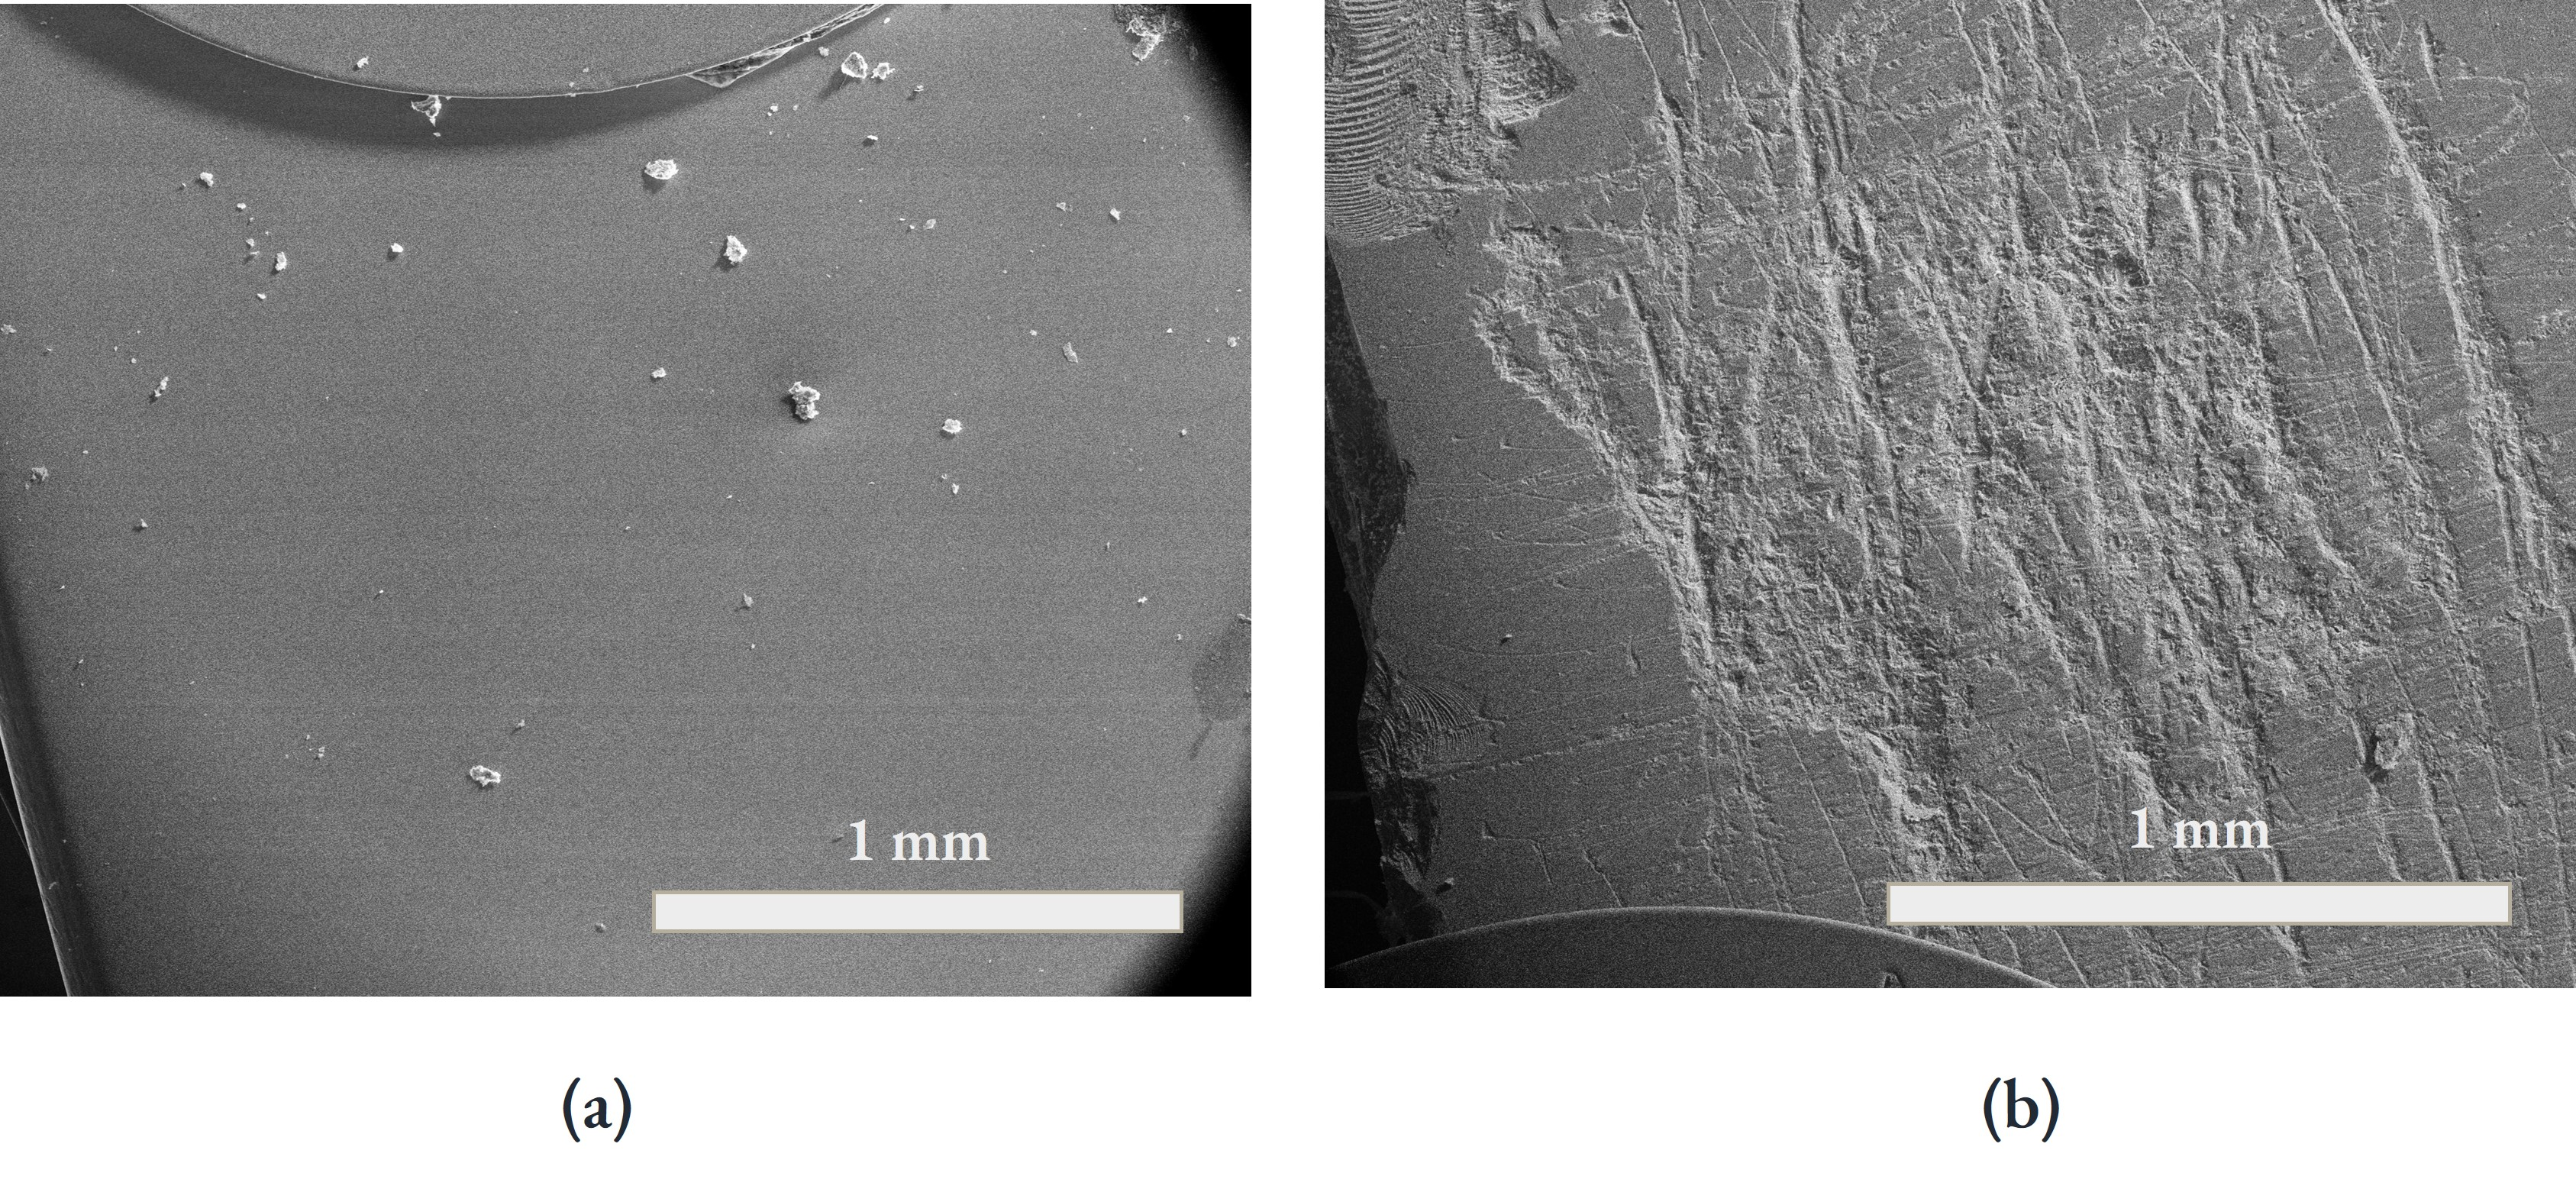
\includegraphics[width=.95\textwidth]{figures/SE_images/Overview_GaAs_GaSb.jpg}
    \caption{
        Overview of the GaAs and GaSb specimen.
        The spectra are acquired in the middle of the images.
        Panel (a) is GaAs, and panel (b) is GaSb.
        The Cu TEM grid is visible at the top and bottom of the images as the large circular object.
        The GaSb wafer have areas which are very scratched, but also areas which are smooth.
    }
    \label{fig:SE_images:Overview_GaAs_GaSb}
\end{figure}

\begin{figure}[htbp]
    \centering
    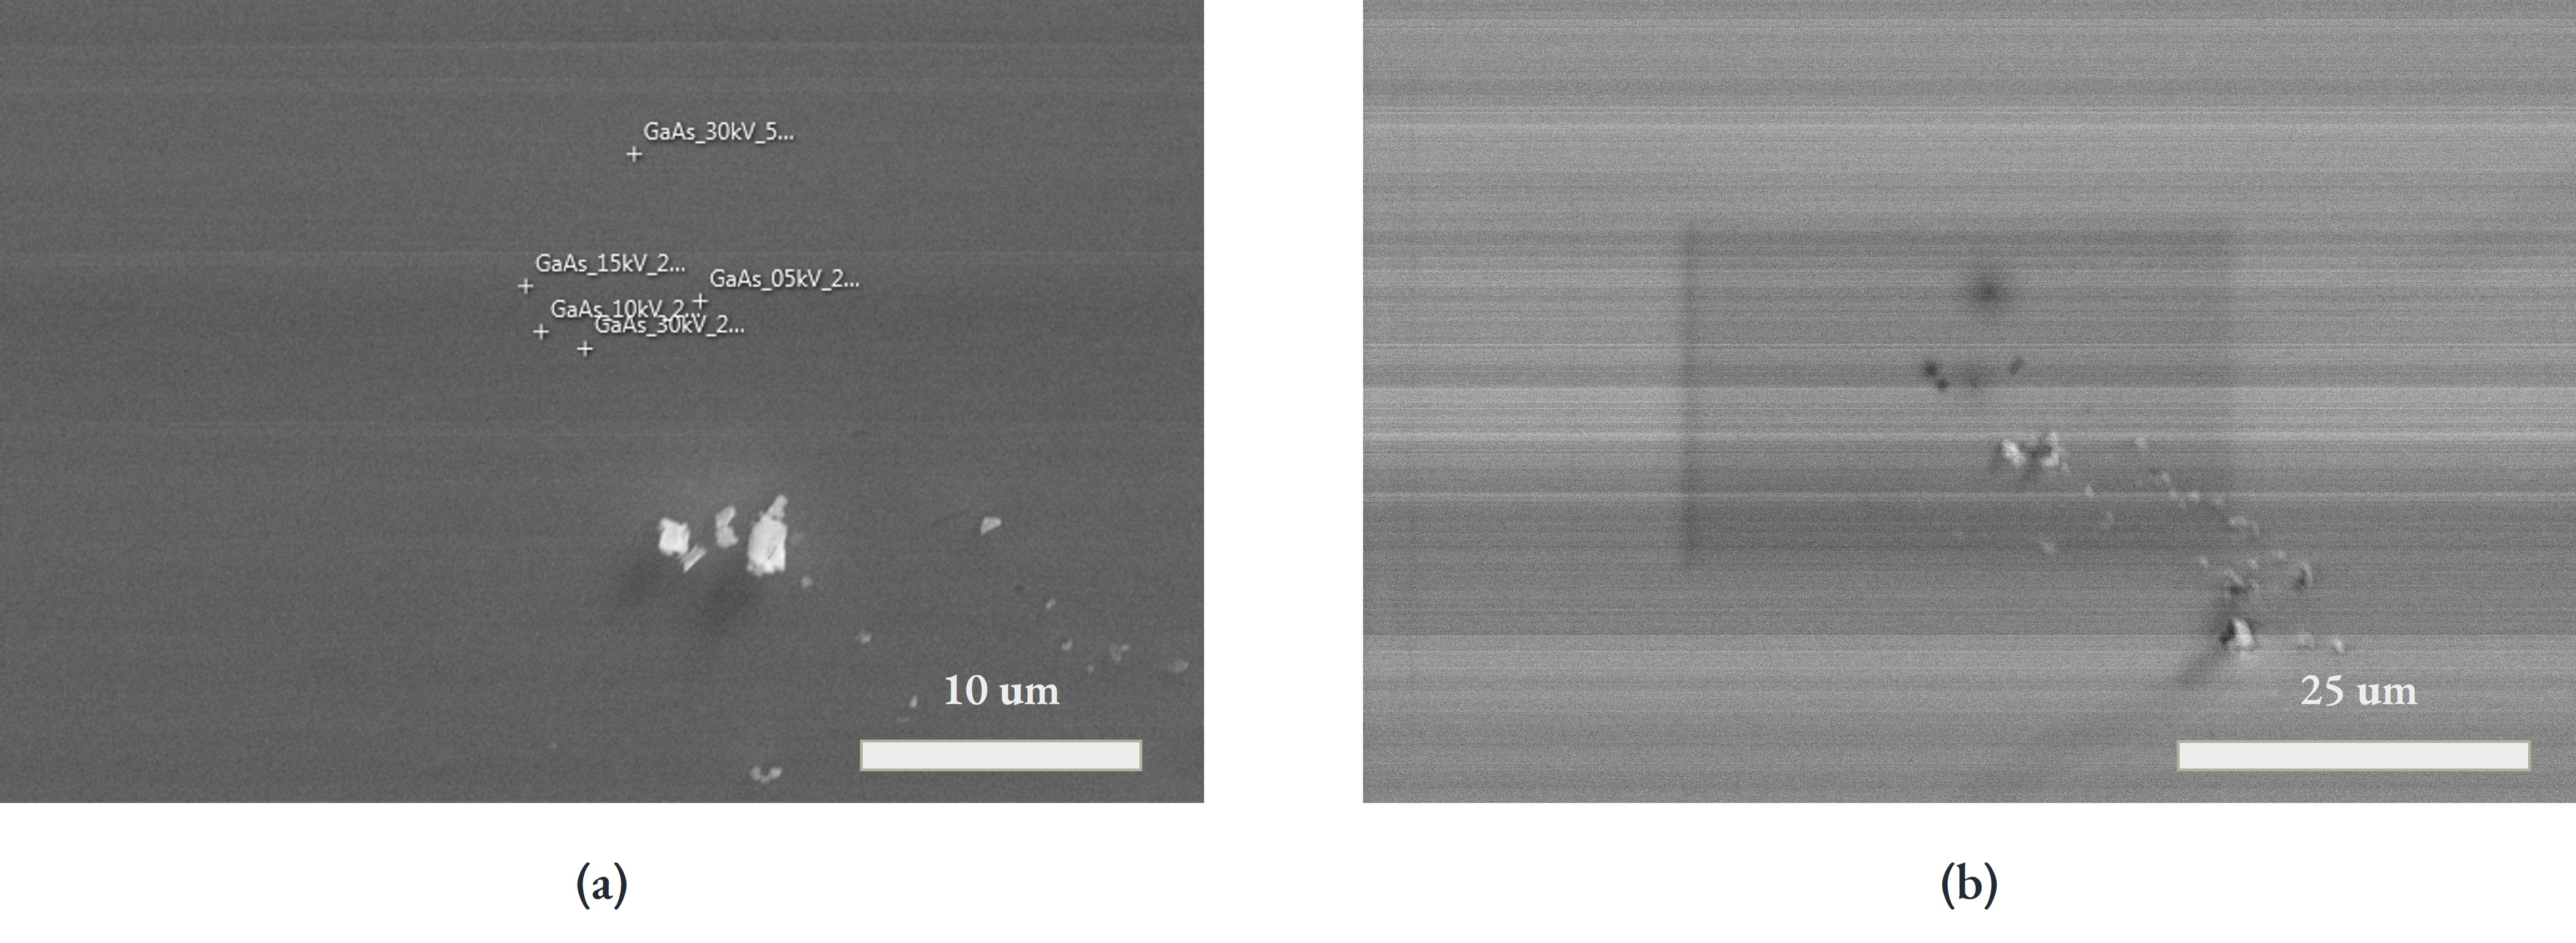
\includegraphics[width=.95\textwidth]{figures/SE_images/GaAs_close.jpg}
    \caption{
        Close up of the GaAs specimen.
        Annotated in panel (a) are the areas which were analyzed.
        Panel (b) is a zoomed out view of the area in panel (a), after the spectra have been acquired.
        This image shows both beam damage from the focused probe beam as black dots, and the whole area from the scanning of the probe beam.
    }
    \label{fig:SE_images:GaAs}
\end{figure}


\begin{figure}[htbp]
    \centering
    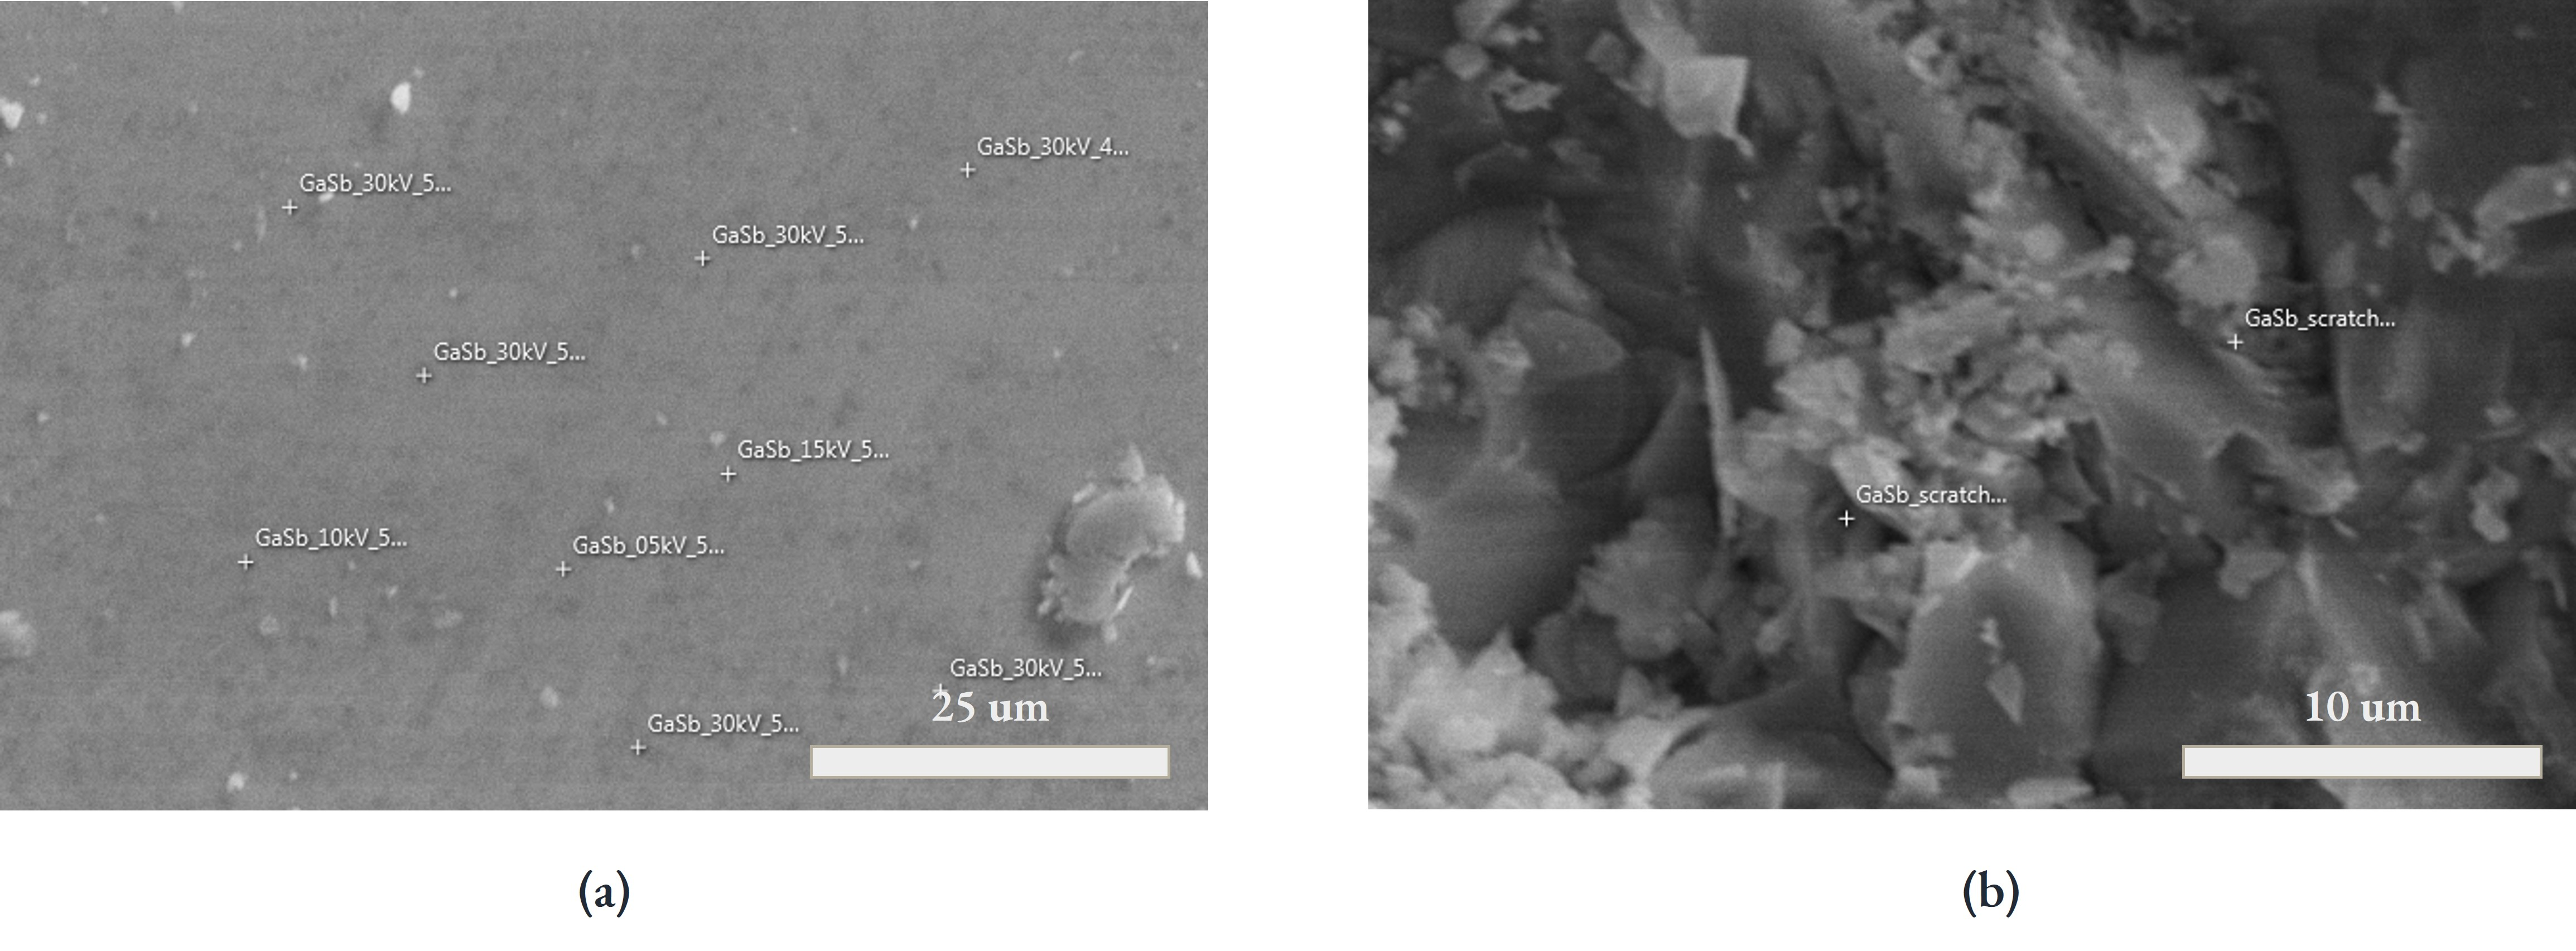
\includegraphics[width=.95\textwidth]{figures/SE_images/GaSb_close.jpg}
    \caption{
        Close up of the GaSb specimen, where the point spectra were acquired.
        Panel (a) is the polished area, and panel (b) is the scratched area.
        Both panels are annotated with the areas which were analyzed.
    }
    \label{fig:SE_images:GaSb}
\end{figure}


% \begin{figure}[htbp]
%     \centering
%     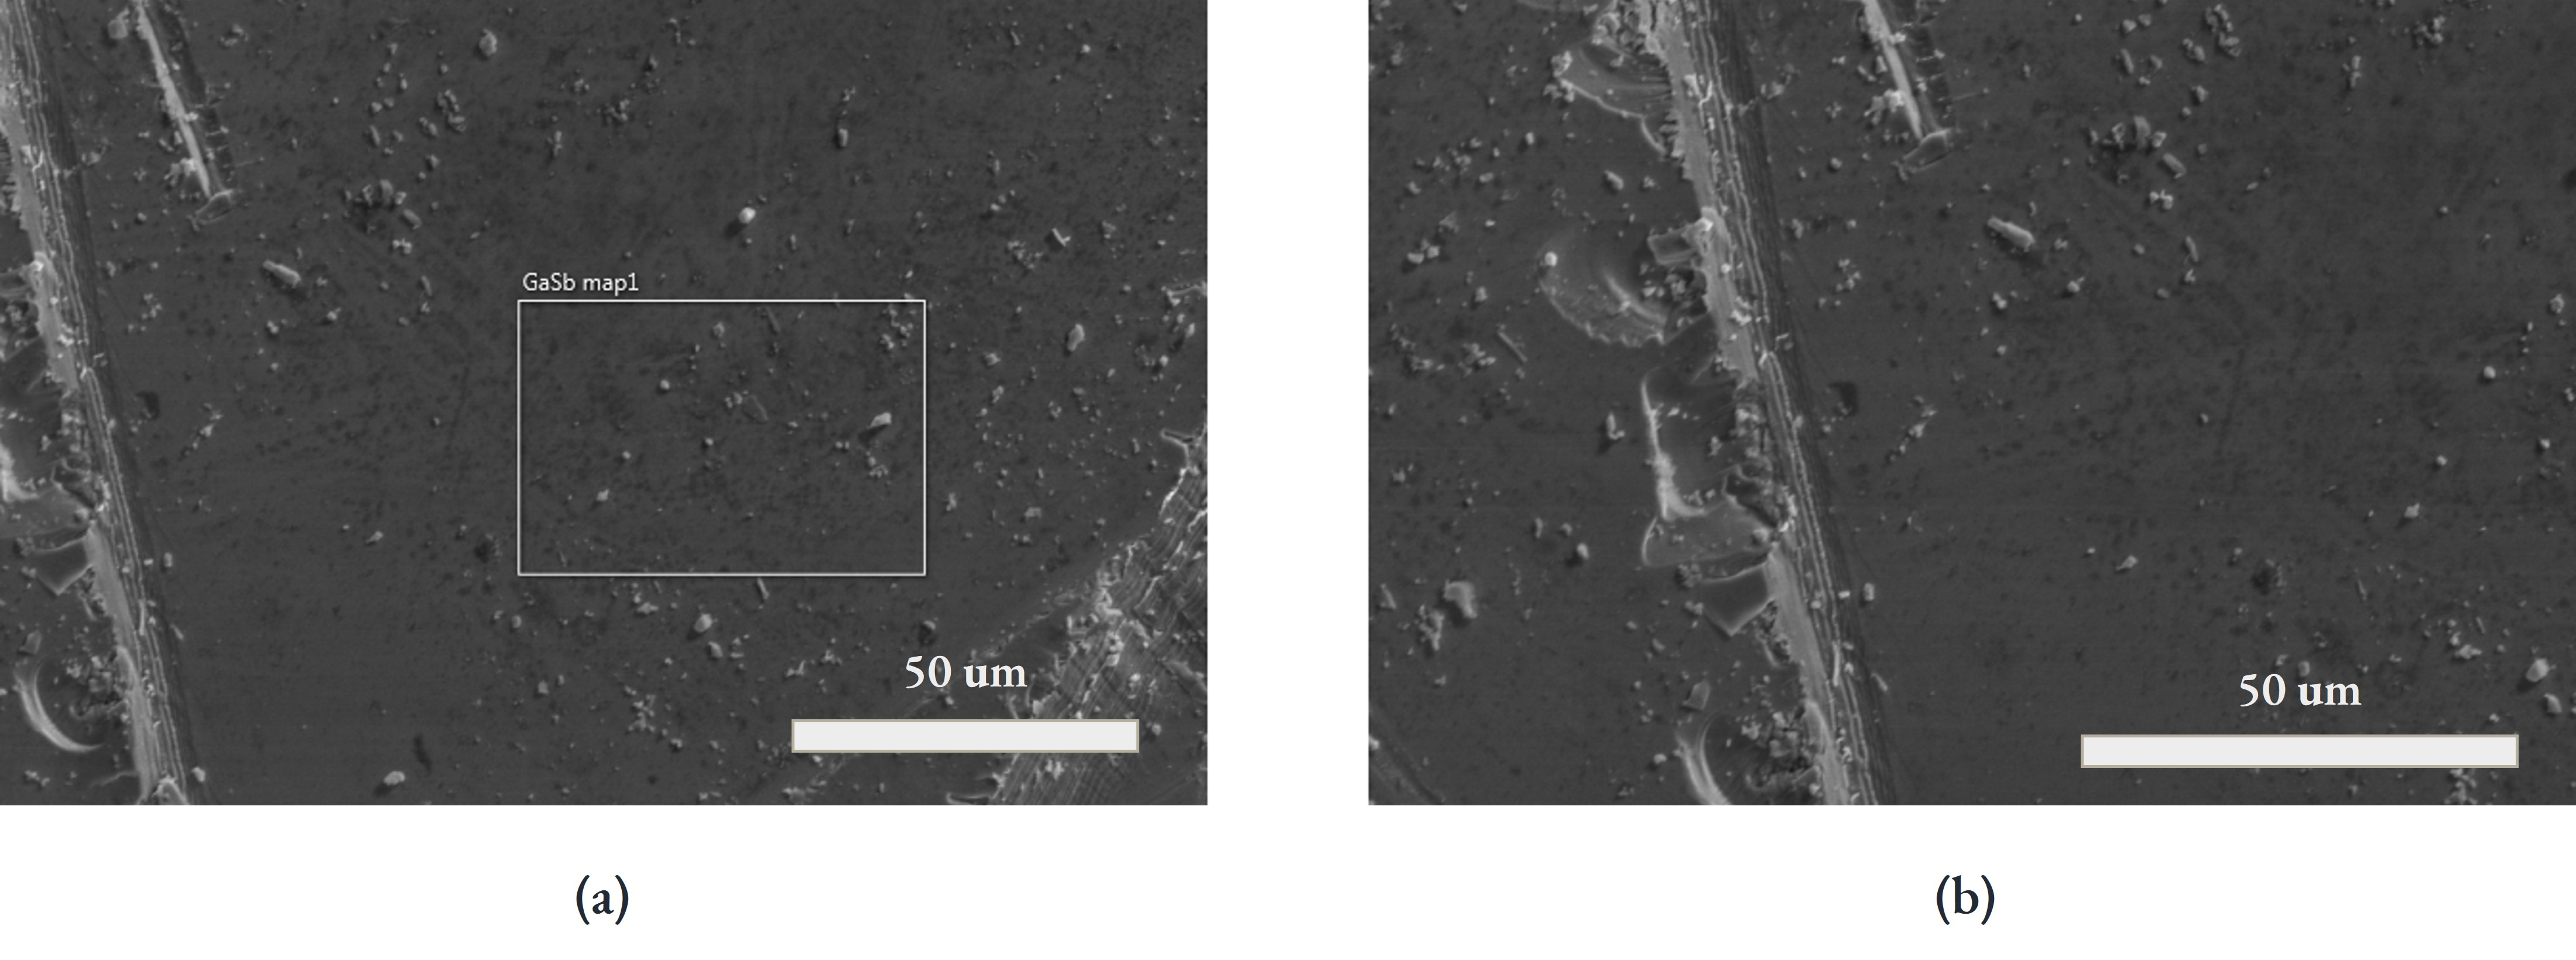
\includegraphics[width=.95\textwidth]{figures/SE_images/GaSb_map.jpg}
%     \caption{
%         Close up of the GaSb specimen, where the map spectra were acquired.
%         Panel (a) is map 1 (within the rectangle), and panel (b) is map 2 (the whole image).
%         Map 2 includes one scratched line in the analyzed area.
%     }
%     \label{fig:SE_images:GaSb_map}
% \end{figure}




\section{Instruments}
\label{method:instruments}

The acquisition of the spectra was done with an Oxford Instruments Xmax$^N$ 80 mm$^2$ silicon drift detector for EDS, equipped on a SEM Apreo from FEI.
\brynjar{TODO from Ton: "Check theory part if all relevant parameters stated there, are listed here." [Relevant parameters of the detector.]}
The Apreo is a field emission SEM, which in addition to the EDS sensor has a Everhart-Thornley detector, in-lens detectors for SE and BSE, a directional BSE detector, and a navigation camera.
In this work, the ET detector was used to verify that the areas studied were clean, flat and representative.
The maximum accelerating voltage is 30 kV, and the maximum beam current is 400 nA.
During this work, the acceleration voltage has been in the range 5-30 kV, and the beam current has been in the range 25-400 pA.
The acquisition settings used in this study are listed in \cref{tab:method:acquisition_settings:voltage} and \cref{tab:method:acquisition_settings:other}.
The instrument is located at the NTNU NanoLab, a NorFab facility.
\brynjar{Cite NorFab?}

\brynjar{The detector is XMAX-N, not just XMAX.}
The details about the EDS detector is from \cite{oxford_xmax_80} and the description provided by NanoLab.
The Oxford Xmax$^N$ SDD has an 80 mm$^2$ active area, which gives a solid angle of 0.03409 sr at WD=10 mm.
The detector is from before 2010, with a claimed count rate of > 500,000 cps and throughout > 200,000 cps \cite{oxford_xmax_80}.
The specifications list an energy resolution of 127 eV, with typical FWHM(Mn K$\alpha$) of 125 eV.
The specified resolution is in compliance with the ISO 15632:2002 standard, the older version of \cite{iso_qc_15632}.
All elements from Be to Pu can be analyzed.
The detector is mounted at 35\textdegree.
The process time settings range from 1 to 6, and they have no further explanation of what the number indicates.
The detector is operated with the AZtec software, provided by Oxford Instruments NanoAnalysis \cite{aztec_manual}.



\section{Acquisition settings in the measurement series}
\label{method:acquisition_settings}

The settings selected are based on Goldstein \cite{goldstein_scanning_2018} and the parameters which was going to be analyzed.
The acquisition is divided into five groups, where the two first are acquisition with varying acceleration voltage and constant beam current.
(A) is the voltage series on GaAs, and (B) is the voltage series on GaSb.
The three last series test other parameters on the GaSb specimen: (C) is with varying PT, (D) is with varying $i_b$ and PT. %, and (E) is data taken with maps.
The voltage series is used to study the effect of the acceleration voltage, to figure out if an optimal voltage exists.
The other acquisition settings tested variations of different settings on the GaSb specimen, to see if any of these settings could improve the quality of the spectra.
The acquisition settings are listed in \cref{tab:method:acquisition_settings:voltage} and \cref{tab:method:acquisition_settings:other}.
An overview of all acquisition settings for each spectrum is given in \cref{tab:method:acquisition_settings:all_spectra}.
Dead time (DT) and input count rate (ICR) is a function of the other settings.


% constant variables
Some variables were kept constant during all the acquisition.
The tilt of the specimen was kept at 0\textdegree, and thus the TOA was 35\textdegree, because of the detector mounting.
The live time for each spectrum was 120 s, except for two of the spectra in the (D) series, which had a high DT.
The range of the spectra was 0-20 keV, with a scale of 10 eV/channel.


\begin{table}[phtb]
    \begin{center}
        \caption{
            Measurement series A and B, which tested different $E_0$ on GaAs and GaSb.
            All spectra were recorded with 0-20 keV energy range and 2048 channels at working distance 10 mm (optimal for the detector), and the at TOA 35\textdegree.
            %
        }
        \renewcommand*{\arraystretch}{1.2}
        \label{tab:method:acquisition_settings:voltage}
        \begin{tabular}{p{2cm}p{3cm}p{8.6cm}}
            \hline
            \textbf{Setting}    & \textbf{Values}      & \textbf{Comment}                                                                                                                                                                                                                                               \\
            \hline
            Beam energy         & 30, 15, 10, and 5 kV & To study the effect of different $E_0$.                                                                                                                                                                                                                        \\
            % Beam current        & 25 pA (GaAs), 50 pA (GaSb) & Set to get sufficient amount of counts and maximum DT around 30\% at 30 kV. Then kept constant when $E_0$ was decreased in the voltage series. Different beam current for the specimen was chosen to see the effects on Ga. \\
            Beam current        & 25 pA or 50 pA       & 25 pA for GaAs and 50 pA for GaSb. Set to get sufficient amount of counts and maximum DT around 30\% at 30 kV. Then kept constant when $E_0$ was decreased in the voltage series. Different beam current for the specimen was chosen to see the effects on Ga. \\
            Process time        & 6 (maximum)          & Set to the highest to influence the acquisition as little as possible, i.e. giving the highest energy resolution.                                                                                                                                              \\
            DT GaAs             & 25\%, 12\%, 6\%, 3\% & DT is not a setting, but a result of other settings. The low DT at the lower $E_0$ was due to fewer counts.                                                                                                                                                    \\
            DT GaSb             & 44\%, 18\%, 9\%, 4\% &                                                                                                                                                                                                                                                                \\
            Data type           & PointID              & The voltage series was only done with PointID, while mapping was tested in the measurement series summarized in \cref{tab:method:acquisition_settings:other}.                                                                                                  \\
            Live time           & 120 s                & To get sufficient amount of counts.                                                                                                                                                                                                                            \\
            Additional spectrum & GaAs, 30 kV, 50 pA   & An additional spectra on GaAs with the same settings at the 30 kV spectrum of GaSb. Taken to directly compare the 30 kV spectra.                                                                                                                               \\

            \hline
        \end{tabular}
    \end{center}
\end{table}
%%%%%%%%%%%%%%%%%%%%%%%%%%%%%%%%%%%%%%%%%%%%%%%%%%%%%%%%%%%%%%%%%%%%%%%%%%%%%%%%%%%%%%%%
%%%%%%%%%%%%%%%%%%%%%%%%%%%%%%%%%%%%%%%%%%%%%%%%%%%%%%%%%%%%%%%%%%%%%%%%%%%%%%%%%%%%%%%%
%%%%%%%%%%%%%%%%%%%%%%%%%%%%%%%%%%%%%%%%%%%%%%%%%%%%%%%%%%%%%%%%%%%%%%%%%%%%%%%%%%%%%%%%
\begin{table}[phtb]
    \begin{center}
        \caption{
            Measurement series B and C, which tested variation in $i_b$, PT, and $E_0$.
            These measurements were only done on the GaSb specimen.
            Data type, live time, energy range, channels, WD, and TOA as in \cref{tab:method:acquisition_settings:voltage}.
        }
        \renewcommand*{\arraystretch}{1.2}
        \label{tab:method:acquisition_settings:other}
        \begin{tabular}{p{2cm}p{3cm}p{8.6cm}}
            \hline
            \textbf{Setting} & \textbf{Values}     & \textbf{Comment}                                                                               \\
            \hline
            Beam energy      & 15 and 30 kV        & Further inspect the effect of the Sb K-peaks just below 30 kV.                                 \\
            Beam current     & 50, 200, and 400 pA & To study ICR and DTs, with values given in \cref{tab:method:acquisition_settings:all_spectra}. \\
            Process time     & 1, 2, 4, and 6      & To study the effect of PT, e.g. on energy resolution and coincidence events.                   \\
            % Data type        & PointID and Map     & Compare results from a point and a map, with eventual denoising in the map.                    \\
            %  &                     &                                                                                                       \\
            %  &                     &                                                                                                       \\
            %  &                     &                                                                                                       \\
            \hline
        \end{tabular}
    \end{center}
\end{table}



\begin{table}[phtb]
    \begin{center}
        \caption{
            Experimental settings of acquired and used spectra in this work.
            % \brynjar{Comment from Ton: Add a column with spectra names, e.g. A, B, C, D.}
            The spectra are divided into five groups: (A) voltage series GaAs, (B) voltage series GaSb, (C) different PT, (D) different $i_b$, $E_0$, and PT, and (E) maps.
            Parameters not specified are as in \cref{tab:method:acquisition_settings:voltage}.
        }
        \renewcommand*{\arraystretch}{1.2}
        \label{tab:method:acquisition_settings:all_spectra}
        \begin{tabular}{lllllllp{3.5cm}}
            \hline
            \textbf{Group}                     & \textbf{Sample} & \textbf{$E_0$} & \textbf{$i_b$} & \textbf{PT} & \textbf{ICR} & \textbf{DT} & \textbf{Comment}    \\
                                               &                 & [kV]           & [pA]           &             & [k counts]   & [\%]        &                     \\
            \hline
            \emph{GaAs $E_0$ series}           &                 &                &                &             &              &             &                     \\
            A                                  & GaAs            & 5              & 25             & 6           & 0.88         & 3           &                     \\
            A                                  & GaAs            & 10             & 25             & 6           & 1.75         & 6           &                     \\
            A                                  & GaAs            & 15             & 25             & 6           & 3.3          & 12          &                     \\
            A                                  & GaAs            & 30             & 25             & 6           & 8            & 25          &                     \\
            A                                  & GaAs            & 30             & 50             & 6           & 16.4         & 44          & Additional spectrum \\
            \hline
            \emph{GaSb $E_0$ series  }         &                 &                &                &             &              &             &                     \\
            B                                  & GaSb            & 5              & 50             & 6           & 1.08         & 4           &                     \\
            B                                  & GaSb            & 10             & 50             & 6           & 2.3          & 9           &                     \\
            B                                  & GaSb            & 15             & 50             & 6           & 5.7          & 18          &                     \\
            B                                  & GaSb            & 30             & 50             & 6           & 17           & 44          &                     \\
            \hline
            \emph{PT change}                   &                 &                &                &             &              &             &                     \\
            C                                  & GaSb            & 30             & 50             & 4           & 17           & 13          &                     \\
            C                                  & GaSb            & 30             & 50             & 2           & 17           & 7           &                     \\
            C                                  & GaSb            & 30             & 50             & 1           & 17           & 4           &                     \\
            \hline
            \emph{$i_b$, $E_0$, and PT change} &                 &                &                &             &              &             &                     \\
            D                                  & GaSb            & 30             & 400            & 1           & 160          & 28          & Very high counts    \\
            D                                  & GaSb            & 15             & 200            & 6           & 22           & 53          & 61 s live time      \\
            D                                  & GaSb            & 15             & 400            & 6           & 42           & 77          & 59 s live time      \\
            %             & GaSb            & 15             & 400             & 3           & 50           & 25          & Scratched area      \\
            %             & GaSb            & 30             & 25              & 6           & 6.5          & 20          & Scratched area      \\
            % \hline
            % \emph{Maps}                &                 &                &                &             &              &             &                     \\
            % E                          & GaSb            & 15             & 400            & 3           & 43           & 22          & Map 1               \\
            % E                          & GaSb            & 15             & 400            & 3           & 43           & 22          & Map 2               \\
            \hline
        \end{tabular}
    \end{center}
\end{table}

































\section{Data treatment}
\label{method:data_treatment}

The data treatment is divided into three parts: acquisition and extraction, performance parameters, and quantification.

\subsection{Acquisition and extraction - AZtec}
\label{method:data_treatment:aztec}

Acquisition and extraction is done with AZtec \brynjar{todo find version}, provided by Oxford Instruments NanoAnalysis \cite{aztec_manual}.
Steps for acquisition is described in Appendix A of Lundeby \cite{lundeby_improving_2019}.
The "SEM EDS" setting was selected.
Point measurements was done with "Point \& ID". 
%, and map measurements was done with "Map".
The point spectra was extracted as ".emsa" files.
% The data from the map spectra was exported as ".emsa", ".raw", ".rpl", and ".txt" files, which was merged to one ".hdf5" file with the script from Lundeby \cite[A.3]{lundeby_improving_2019}.
% The merge script and the relevant Appendix from Lundeby is available at the author of this thesis' GitHub \verb|\cref{} or link|.

Summarized, the acquisition and extraction in AZtec was done as follows:
\begin{enumerate}
    \item "SEM EDS" setting selected.
    \item Data type selected as "Point \& ID".
    \item Navigated to the area of interest with the ET detector.
    \item Selected settings for the acquisition, see \cref{tab:method:acquisition_settings:all_spectra}.
    \item Started the acquisition.
    \item Verified the element with the spectrum and an interactive periodic table.
    \item AZtec calculated the composition.
    \item The spectra were extracted for notebook analysis.
\end{enumerate}


Initial qualitative analysis was done with the AZtec software, to get an overview of the spectra.
All spectra were quantitatively analyzed with the AZtec software to later compare with HyperSpy and the notebooks developed in this thesis.
The "SEM EDS" quantification in AZtec give the composition and the calculated k-ratios for each element.
Additionally, quantification with the "TEM EDS" setting in AZtec was tested, where both the composition and calculated k-factors were extracted.
This "TEM EDS" step was done to verify that AZtec does use matrix corrections, and to get the k-factors for quantification with HyperSpy.
\brynjar{TODO discussion: the TEM treatment was expected to yield poor results, which it did.}



\subsection{Performance parameters - Jupyter notebooks}
\label{method:data_treatment:notebook}

Two Jupyter notebooks were developed as a part of this work for the analysis of SEM EDS performance parameters, i.e. the top and middle row of \cref{fig:intro:parameters}.
The notebooks for performance parameters calibrates the spectrum, and calculates: the Duane-Hunt limit, the energy resolution, the Fiori P/B, peak intensities, FWHMs, peak deviations, and specified peak ratios.
The notebooks for quantification is described in \cref{method:data_treatment:quantification}.


All the notebooks run on Python 3.10, with the packages listed in \cref{tab:method:packages}.
All dependencies were installed using the package manager Mamba 1.4.0, with Conda 22.11.1.
When contributing to HyperSpy, the developer version of HyperSpy was installed using pip 23.0.
The notebooks are both attached in the appendix of this thesis, and available at the author of this thesis' GitHub \verb|TODO: \cref{} or link|.
Two first notebooks is for analysis of a single spectrum with a ".csv" output, and second is one for statistics on a set of outputted ".csv" files.

\begin{table}[hbtp]
    \begin{center}
        \caption{
            The Python packages.
            All dependencies was installed using the package manager Mamba 1.4.0, with Conda 22.11.1.
            When contributing to HyperSpy, the developer version of HyperSpy was installed using pip 23.0.
        }
        \renewcommand*{\arraystretch}{1.2}
        \label{tab:method:packages}
        \begin{tabular}{p{4cm}p{10.6cm}}
            \hline
            \textbf{Package name} & \textbf{Description}                                          \\
            \hline
            HyperSpy 1.7.4        & Multi-dimensional data analysis toolbox.                      \\
            Plotly 5.13.1         & Interactive, open-source, and browser-based graphing library. \\
            Numpy 1.23.5          & Scientific computing with Python.                             \\
            Pandas 1.5.3          & Data analysis package.                                        \\
            JupyterLab 3.6.2      & Web-based interactive development environment.                \\
            SciPy 1.10.1          & Scientific computing with Python.                             \\
            Matplotlib 3.7.1      & Static, animated, and interactive visualizations.             \\
            \hline
        \end{tabular}
    \end{center}
\end{table}




The performance parameter notebook does the following steps:

\begin{enumerate}
    \item Import the packages
    \item Import the data with HyperSpy, and set the elements in the spectrum
    \item Set the variables like the beam current, acceleration voltage, ICR, and PT for the output
    \item Slice off the noise peak
    \item Calculate the Duane-Hunt limit, and slice the spectrum to the limit
    \item Make a model of the spectrum, with the background as a polynomial and the peaks as Gaussian functions
    \item Fit the background, then fit the whole model
    \item Calibrate the offset and scale
    \item Calibrate the energy resolution
    \item Calibrate the energy and width of the peaks
    \item Calculate Fiori P/B, peak intensities, FWHMs, and peak deviations
    \item Calculate the relevant peak ratios
          % \item Calculate the relavant FWTM/FWHM 
    % \item Calculate the total count statistics
    \item Visualization of the results
    \item Make a DataFrame with the results and output it as a ".csv" file
\end{enumerate}

\brynjar{TODO from Ton: "These are headers, have them in the notebook as headers.
    This listing is for reader not so informative. Suggestions: Could have behind each link to theory "(section 2.x, specifically implementation of eq. 2.x)". The main content is in the notebooks in the appendix. To list all here makes them unreadable, reader need to use appendix and notebook needs headers and comments to have it readable.
    When linking parts by referring have same phrasing and numbers/labels."}


The statistics notebook loads the wanted ".csv" files into Pandas DataFrames, which are then used to calculate the statistics and look at differences in the metrics.
Some data is plotted, some are shown in tables.


























\subsection{Quantification - HyperSpy and Jupyter notebooks}
\label{method:data_treatment:quantification}


Intro \dots

\brynjar{TODO: Unfinished. I use PAP or XPP, this section comes when the notebook is more finished.}



